\documentclass[oneside,a4paper,11pt]{book} 
\setcounter{secnumdepth}{4}
\setcounter{tocdepth}{4}   
\usepackage{fancyhdr}
\setlength{\headheight}{15pt}
\usepackage[pdftex,
pdfauthor={Name, Vorname},
pdftitle={Überschrift},
pdfsubject={Projektarbeit},
pdfkeywords={Unterschrift}
]{hyperref}
\usepackage[ngerman]{babel}
\usepackage[T1]{fontenc}
\usepackage[utf8]{inputenc}
\usepackage[dvips]{graphicx}
\usepackage{calc}
\usepackage{makeidx}
\usepackage{xcolor}
\usepackage[hang,small,scriptsize,bf]{caption}
\usepackage{hsel-thesis2020}
\usepackage{amssymb}
\usepackage{subcaption}
\usepackage{hyperref}
\usepackage{multirow}
\usepackage{circuitikz}
\usepackage{seqsplit}
\usepackage{csquotes}
\usepackage{makecell}
\usepackage{animate}
\usepackage{eso-pic}
\usepackage{newfloat}
\usepackage{pdfpages}
\usepackage{tikz}
\usepackage{listings}
\usepackage[normalem]{ulem}
\usepackage[
  style=numeric,
  sorting=none,
  backend=biber
  ]{biblatex}
\addbibresource{Literaturverzeichnis.bib}
\usetikzlibrary{positioning}


\newcommand{\myboxy}[3]{
	\begin{tikzpicture}[
			every node/.style={rectangle,rounded corners,draw=black, top color=white,very thick, inner sep=0.3em, minimum size=1em} ]
		\node[text width=#3](main) at (0,0 ){\vspace{3pt}  #1};
		\node[above =-2mm of main.north west, anchor=south west] (title) {#2};
	\end{tikzpicture} }



\newcommand{\textbfit}[1]{\textbf{\textit{#1}}}




\DeclareFloatingEnvironment[
	listname  = {Diagrammverzeichnis}, % Listenüberschrift
	name      = Diagramm,              % Name in Beschriftungen
]{scheme}


\DeclareFloatingEnvironment[
	listname  = {Oszillogrammverzeichnis}, % Listenüberschrift
	name      = Oszillogramm,              % Name in Beschriftungen
]{oszillo}


%%%%%%%%%%%%%%%%%%%%%%%%%%%%%%%%%%%%%%%%%%%%%%%%%%%%%%%%%%%%%%%%%%%%%%%%%%%%%%%%%%%%
%%%%%%%%%%%%%%%%%%%%%%%%%%%%%%%%%%%%%%%%%%%%%%%%%%%%%%%%%%%%%%%%%%%%%%%%%%%%%%%%%%%%
%%%%%%%%%%%%%%%%%%%%%%%%%%%%%%%%%%%%%%%%%%%%%%%%%%%%%%%%%%%%%%%%%%%%%%%%%%%%%%%%%%%%
%%%%%%%%%%%%%%%%%%%%%%%%%%%%%%%%%%%%%%%%%%%%%%%%%%%%%%%%%%%%%%%%%%%%%%%%%%%%%%%%%%%%
%%%%%%%%%%%%%%%%%%%%%%%%%%%%%%%%%%%%%%%%%%%%%%%%%%%%%%%%%%%%%%%%%%%%%%%%%%%%%%%%%%%%
%%%%%%%%%%%%%%%%%%%%%%%%%%%%%%%%%%%%%%%%%%%%%%%%%%%%%%%%%%%%%%%%%%%%%%%%%%%%%%%%%%%%


\begin{document}
\allsectionsfont{\sffamily}


\AddToShipoutPicture{\BackgroundWave}
\pagenumbering{Roman}

\begin{titlepage}

	\vspace{-0.5cm}
	\hspace{-3.0cm}
	% \hspace{-2.0cm}
	\begin{tabular}{p{8.0cm} p{8.0cm}}
		
\includegraphics[width = 6.0cm]{img/GUI/hsel-allgemein} &
		\parbox[b]{8.0cm}{
		{\large 	Fachbereich Technik }                            \\
		{\large 	Abteilung Elektrotechnik und Informatik }
		}                                                         \\
		\\
		\hline
	\end{tabular}
	%
	\begin{center}

		\vspace{2.5cm}
		\LARGE{\textsc{
				Hyperloop\\
				48 V
			}}\\

		\vspace{2.5cm}
		\LARGE{\textsc{
				{Projektarbeit}
			}}\\
		\large
		Studiengang Elektrotechnik

		\vspace{2cm}%
		\large
		Vorgelegt von\\ Oliver, Schmidt\\ Studiengang Elektrotechnik\\ Matr. Nr. 7023462

		\vspace{1cm}
		Emden, \today

		\vspace{3.5cm}%
		Betreut von\\ Prof. Dr.-Ing. Kane

	\end{center}
	\normalsize
\end{titlepage}

\linespread{1.2}
\noitemsep
\include{source/0_1_RechtlicheErklärung}
\tableofcontents
\listoffigures
\label{sec:Abbildungsverzeichnis}
\addcontentsline{toc}{section}{Abbildungsverzeichnis}



\listoftables
\label{sec:Tabellenverzeichnis}
\addcontentsline{toc}{section}{Tabellenverzeichnis}

\listofscheme
\label{sec:Diagrammverzeichnis}
\addcontentsline{toc}{section}{Diagrammverzeichnis}

\listofoszillo
\label{sec:Oszillogrammverzeichnis}
\addcontentsline{toc}{section}{Oszillogrammverzeichnis}



%\lstlistoflistings
%\label{sec:Codeverzeichnis}
%\addcontentsline{toc}{section}{Code Listings}

\newpage


\cleardoublepage
\pagenumbering{arabic}
\ClearShipoutPicture

\chapter{Einleitung}
\label{chapter:Einleitung}

\section{Motivation}
\label{section:Motivation}

Der Hyperloop ist ein innovatives Transportkonzept, das eine ökonomische, klimafreundliche und schnellere Alternative zu herkömmlichen Verkehrsmitteln wie Lastkraftwagen, Zügen und Flugzeugen bietet.
Derzeit stehen herkömmlichen Transportmitteln zwei wesentliche Hindernisse im Weg, um Personen und Güter schnell und emissionsarm zu befördern: Zum einen der hohe Luftwiderstand, der bei hohen Geschwindigkeiten den Energieverbrauch stark erhöht, und zum anderen der Rollwiderstand der Räder, der ebenfalls zu einem höheren Energiebedarf führt.
\begin{figure}[!ht]
	\begin{center}
		\includegraphics[width=1\textwidth]{img/1_strecke/strecke_1.png}
		\caption{Hyperloop der Hochschule Emden-Leer}
		\label{img_1_1:strecke}
	\end{center}
\end{figure}
\pagebreak[1]


Der Hyperloop löst diese Probleme, indem er Güter und Personen in einem Fahrzeug, das sich in einer Vakuumröhre bewegt, wie in Abbildung \ref{img_1_1:strecke} dargestellt ist, zudem wird das Fahrzeug, wie bei einer Magnetschwebebahntechnik angehoben, somit lassen sich Roll- und Luftwiderstand fast vollkommen aufheben.

Angesichts der globalen Bemühungen zur Reduzierung der CO2-Emissionen und zur Bekämpfung des Klimawandels könnte Hyperloop eine umweltfreundlichere Alternative zu Autos und Flugzeugen bieten.





\subsection{Institute of Hyperloop Technology}
\label{section:IHT}

\textbf{\textcolor{red}{Zitieren!!!!!!}}\\ \ \\
Die Hochschule Emden/Leer hat im Jahr 2021 das Institut für Hyperloop-Technologie (IHT) gegründet, um aktiv an der Forschung zu dieser zukunftsweisenden Technologie teilzunehmen.

Im Rahmen dieser Forschung wurde an der Hochschule Emden eine Teststrecke mit einer Länge von 26 Metern errichtet (siehe Abbildung \ref{img_1_1:strecke}). Auf dieser Strecke soll das Fahrzeug (POD) unter realistischen Bedingungen getestet und weiterentwickelt werden.
Die Teststrecke besteht aus einem Schinensystem und einem Linarmotor. Der Linarmotor wird für die Magnetschwebebahntechnik verwendet.


Darüber hinaus engagiert sich das IHT in verschiedenen Projekten, darunter das \frqq European Hyperloop Technology Center – EuHyTeC\flqq, das europäische Hyperloop-Initiativen vernetzt und gemeinsam die nächste Generation des Transports entwickelt.
\newpage




\section{Aufgabenstellung}
\label{section:Aufgabenstellung}

\myboxy{
	\begin{itemize}
		\item Ablauforientiert erklären. Also erst die Bestellung, dann der Schaltplan und dann die Simulation mit Simulink.
		\item Aufgabenstellung in der Vergangenheit formulieren.
		\item Den Leser in der Doku struktur Einführen. Am enden in 1.x
	\end{itemize}
}{To-do}{\textwidth}


Die Motivation für dieses Projekt liegt in der Entwicklung eines Hyperloop-Fahrzeugs, das mit einer Batterie und einem Motor betrieben wird. Für die Steuerung des Fahrzeuges wurde ein echtzeitfähiges Steuerungsystem der Firma Speedgoat vorgeben, welches in Abschnitt \ref{section:speedgoat} vertieft wird.\\ \ \\

Im Rahmen des Projekts wird ein Fahrzeug (Pod) für den Hyperloop mit einer Bordspannung von 48 V konzipiert. Ziel ist es, die Machbarkeit dieser Spannung zu überprüfen und umzusetzen. Dazu gehören die Planung und Simulierung, die Integration der erforderlichen Sensorik sowie die Beschaffung der notwendigen Bauteile. Die Logik- und Signalverarbeitung wird mithilfe von Simulink auf dem echtzeitfähigen Speedgoat-System durchgeführt.
Die Steuerung erfolgt über Simulink, ein Modul von MATLAB, und umfasst die Erfassung von Position und Beschleunigung des Fahrzeuges. Der Motor wird über ein zusätzliches Steuergerät angesteuert. Die Steuerung soll als Automatensteuerung umgesetzt werden.
Die Verdrahtung des Pods wird entsprechend der Bordspannung von 48 V ausgelegt. Hierfür wird mit der Software QElectroTech ein Schaltplan erstellt.
Alle erforderlichen Bauteile für die Umsetzung der Bordspannung, die Verdrahtung und die Sensorik müssen beschafft werden.
Textergebnisse und in Betriebnahme entfallen.


\section{Aufbau der Projektdokumentation}
\label{section:Aufbau}

\chapter{Bonusmaterial}
\label{sec:Anhang}

\chapter{Konzept}
\label{chapter:Konzept}

Wie in Abbildung \ref{img_1_1:Konzept:0} dargestellt, werden die Baugruppen des Pods an verschiedenen Stellen miteinander verbunden. Dabei übernimmt die Steuereinheit (+SE1) eine zentrale Rolle. Mit der echtzeitfähigen Steuerung von Speedgoat werden alle digitalen und analogen Ein- und Ausgangssignale gesteuert, einschließlich der Distanzmessung und der G-Kraft-Messungen. Die Distanzmessung ist für die Positionsermittlung notwendig, während die G-Kraft-Messung für Forschungszwecke genutzt werden soll. Die Steuereinheit (+SE1) wird von der Batterieeinheit (+BE2) mit Energie versorgt.

\begin{figure}[!ht]
	\begin{center}
		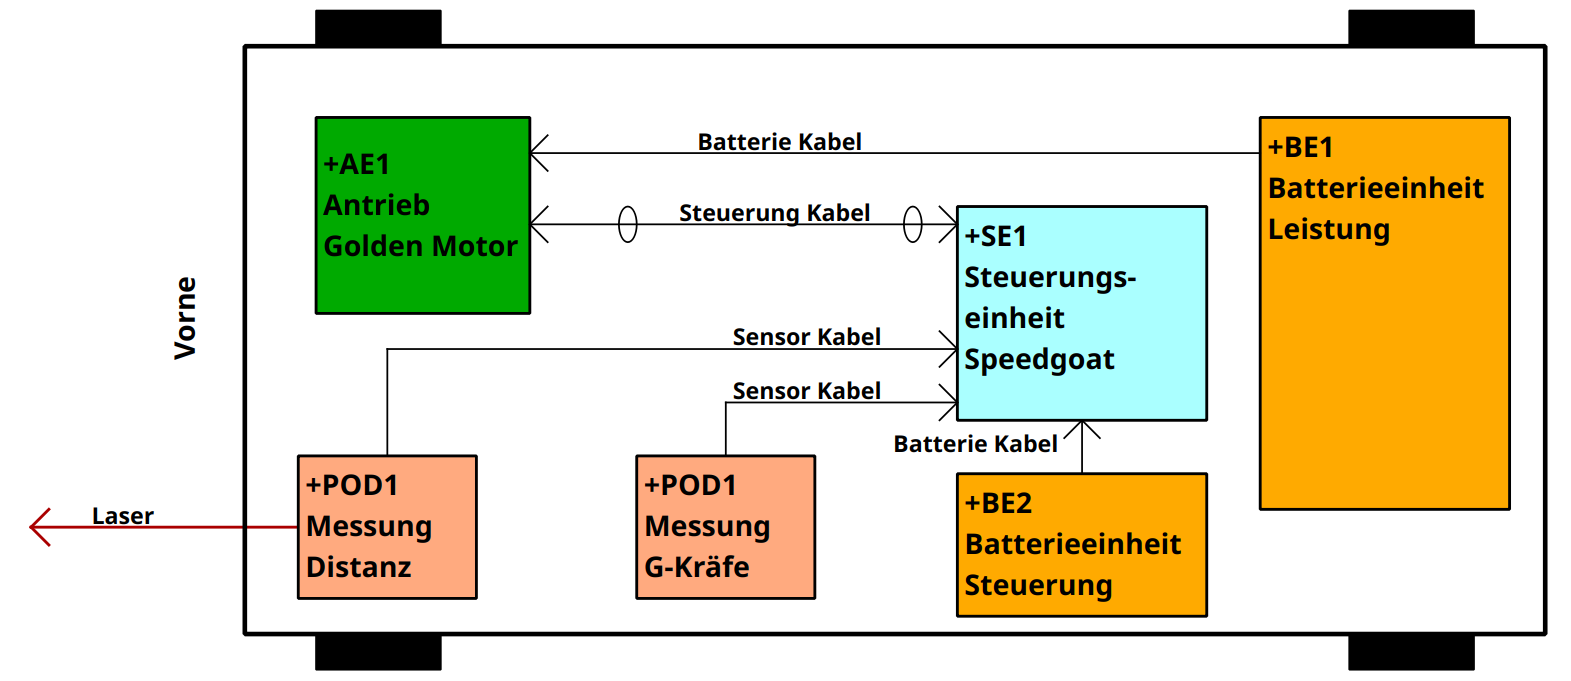
\includegraphics[width=1\textwidth]{img/3_schaltplan/sp_aufbauplan_0.png}
		\caption{Konzept – Aufbauplan des Pods}
		\label{img_1_1:Konzept:0}
	\end{center}
\end{figure}

Der Antrieb (+AE1) erfolgt über einen BLDC-Motor. Dieser wird mittels eines zusätzlichen Steuergeräts, einem Vector-Controller (FOC: Field Oriented Control), angesteuert. Für die Energieversorgung des Antriebs wird eine Leistungsbatterie (+BE1) verwendet.


\chapter{Bonusmaterial}
\label{sec:Anhang}

\chapter{Stand der Technik}
\label{chapter:Stand_der_Technik}
\myboxy{
	\begin{itemize}
		\item Bilder neu machen aus dem Schaltplan.
		\item Vector Controller, Funktionsweise nur kurz erklären und mehr auf die Anschlüsse eingehen.
		\item PIN-Mapping als Tabelle erstellen, für den Motor und den Vector Controller.
		\item QElectroTeck.
		\item PIN-Mapping als Tabelle erstellen, für den Motor und den Vector Controller.
		\item Auf die PDF verweisen.
	\end{itemize}
}{To-do}{\textwidth}



In dem folgenden Abschnitt werden die verwendeten Bauteile, welche in Kapitel \ref{chapter:Konzept} dargestellt worden sind, näher beschrieben.


\section{Antrieb – Golden Motor}
\label{section:Antrieb}

Golden Motor bietet eine Gesamtlösung bestehend aus einem BLDC-Motor und einem Vektor-Controller an. Der Motor wird dabei mit dem Controller verbunden, der eine Schnittstelle mit allen notwendigen Steuer- und Kontrollsignalen bereitstellt, um den Motor anzutreiben. Die Anschlüsse sowie die grundlegende Funktionsweise werden in den Abschnitten \ref{section:BLDC_Motor} und \ref{section:Vector_Controller} näher erläutert.



\subsection{BLDC Motor}
\label{section:BLDC_Motor}


Der in Abbildung \ref{BLDC_Motor:img:antrieb_motor} dargestellte BLDC-Motor verfügt über eine Leistung von 10 kW und kann optional durch eine Ölkühlung gekühlt werden, was jedoch für das Fahrzeug derzeit nicht relevant ist. Die Drehzahl ist variabel und kann zwischen 2.000 und 6.000 U/min eingestellt werden, mittls dem Vector Controller der in Abschnitt \ref{section:Vector_Controller} erklärt wird. Das Nenndrehmoment beträgt 26 Nm, während das maximale Drehmoment bei 85 Nm liegt. Der Wirkungsgrad des Motors beträgt 91 \% \cite{Golden_Motor:bldc_motor}.

\pagebreak[1]
\begin{figure}[!ht]
	\begin{center}
		\includegraphics[width=1\textwidth]{img/2_antrieb/motor_1.png}
		\caption{Golden Motor – 10 KW BLDC Motor Liquid Cooled}
		\label{BLDC_Motor:img:antrieb_motor}
	\end{center}
\end{figure}


Die Anschlüsse des Motors sind in Tabelle \ref{BLDC_Motor:tab:pinmapping} aufgelistet. Der Motor verfügt über zwei Hall-Sensor-Kabel, die jeweils drei Hall-Sensoren sowie einen Temperatursensor enthalten. Zusätzlich sind ein GND- und ein +5V-Versorgungsanschluss in den Hall-Sensor-Kabeln integriert. Die Spulen des Motors werden über sechs separate Kabel angeschlossen: U, V und W.
\pagebreak[1]
\begin{table}[!ht]
	\centering
	\caption{Pin Mapping – BLDC-Motor}
	\label{BLDC_Motor:tab:pinmapping}
	\begin{tabular}{lll}
		\hline
		\textbf{Anschluss}          & \textbf{Funktionalität} & \textbf{Farbe} \\ \hline
		\multicolumn{3}{c}{\textbf{Anschluss Adern Motor}}                     \\ \hline
		\multicolumn{1}{l|}{U1}     & Spule 1                 & Gelb           \\
		\multicolumn{1}{l|}{V1}     & Spule 2                 & Grün           \\
		\multicolumn{1}{l|}{W1}     & Spule 3                 & Blau           \\
		\multicolumn{1}{l|}{U2}     & Spule 1                 & Gelb           \\
		\multicolumn{1}{l|}{V2}     & Spule 2                 & Grün           \\
		\multicolumn{1}{l|}{W2}     & Spule 3                 & Blau           \\ \hline
		\multicolumn{3}{c}{\textbf{Motor Hall Kabel 1}}                        \\ \hline
		\multicolumn{1}{l|}{Hall A} & Hall Sensor             & Gelb           \\
		\multicolumn{1}{l|}{Hall B} & Hall Sensor             & Grün           \\
		\multicolumn{1}{l|}{Hall C} & Hall Sensor             & Blau           \\
		\multicolumn{1}{l|}{Temp}   & Temperatur Sensor       & Weiß           \\
		\multicolumn{1}{l|}{+5V}    & Spannungsversorgung     & Rot            \\
		\multicolumn{1}{l|}{GND}    & Masse                   & Schwarz        \\ \hline
		\multicolumn{3}{c}{\textbf{Motor Hall Kabel 2}}                        \\ \hline
		\multicolumn{1}{l|}{Hall A} & Hall Sensor             & Gelb           \\
		\multicolumn{1}{l|}{Hall B} & Hall Sensor             & Grün           \\
		\multicolumn{1}{l|}{Hall C} & Hall Sensor             & Blau           \\
		\multicolumn{1}{l|}{Temp}   & Temperatur Sensor       & Weiß           \\
		\multicolumn{1}{l|}{+5V}    & Spannungsversorgung     & Rot            \\
		\multicolumn{1}{l|}{GND}    & Masse                   & Schwarz        \\ \hline
	\end{tabular}
\end{table}
\pagebreak[4]



\subsubsection{Funktionsweise}
\label{BLDC_Motor:Funktionsweise}
Ein BLDC-Motor (Brushless DC Motor) unterscheidet sich grundlegend von einem herkömmlichen Gleichstrommotor. Während bei einem traditionellen DC-Motor die Polumschaltung (Kommutierung) mechanisch über Kohlebürsten erfolgt, übernimmt beim BLDC-Motor eine elektronische Steuerung diese Aufgabe. Dadurch entfällt die Notwendigkeit von Kohlebürsten, was den Motor effizienter und langlebiger macht\cite{mathworks:bldc_motor}.
\newpage



\subsection{Vector Controller}
\label{section:Vector_Controller}

Der Motor wird mithilfe eines Vektor-Controllers angesteuert, der in Abbildung \ref{Vector_Controller:img:Antrieb_Controller} dargestellt ist. Der Controller hat die Aufgabe, den Motor basierend auf den Eingangssignalen so zu steuern, dass beispielsweise eine gewünschte Drehzahl erreicht wird. Die genaue Funktionsweise des Vektor-Controllers wird kurz unter \ref{Vector_Controller:Funktionsweise} erläutert.

Das Pin-Mapping ist in Tabelle \ref{Vector_Controller:tab:pinmapping} aufgeführt. Bei den Steuersignalen muss auf den Spannungsbereich geachtet werden, da der Controller eine Störung meldet, wenn ein Signal außerhalb des zulässigen Bereichs liegt. Dies ist ein integriertes Sicherheitssystem des Controllers. Dies ist ein integriertes Sicherheitssystem des Controllers. So liegt beispielsweise bei der Bremse das digitale Signal bei 0, wenn die Spannung 1 V beträgt. Tritt ein Kabelbruch so wird die Spannung am Controller bei 0 V liegen und eine Warnung wird durch ein periodisches Piepen ausgegeben.


\begin{figure}[!ht]
	\begin{center}
		\includegraphics[width=1\textwidth]{img/2_antrieb/sine_1.png}
		\caption{Golden Motor – VECTOR 500 Motor Controller}
		\label{Vector_Controller:img:Antrieb_Controller}
	\end{center}
\end{figure}

\begin{table}[!ht]
	\centering
	\caption{Pin Mapping – Vector Controller}
	\label{Vector_Controller:tab:pinmapping}
	\begin{tabular}{lll|l}
		\hline
		\textbf{Anschluss}           & \textbf{Funktionalität}  & \textbf{Farbe}              & \textbf{U in V}             \\ \hline
		\multicolumn{4}{c}{\textbf{Batterie Eingang}}                                                                       \\ \hline
		\multicolumn{1}{l|}{B+}      & Versorgungsspannung      & RT                          & 48 V                        \\
		\multicolumn{1}{l|}{B-}      & Masse                    & SW                          & 0 V                         \\ \hline
		\multicolumn{4}{c}{\textbf{Motor Ausgnag}}                                                                          \\ \hline
		\multicolumn{1}{l|}{U}       & Spule 1                  & GE                          &                             \\
		\multicolumn{1}{l|}{V}       & Spule 2                  & GN                          &                             \\
		\multicolumn{1}{l|}{W}       & Spule 3                  & BL                          &                             \\ \hline
		\multicolumn{4}{c}{\textbf{Steuerungskabel}}                                                                        \\ \hline
		\multicolumn{1}{l|}{1}       & CANL - CAN-Bus           & \textcolor{red}{Vorhanden?} &                             \\
		\multicolumn{1}{l|}{2}       & CANH – CAN-Bus           & \textcolor{red}{Vorhanden?} &                             \\
		\multicolumn{1}{l|}{3}       & Motor Temperatur         & BL                          &                             \\
		\multicolumn{1}{l|}{4, 5, 6} & Masse                    & SW                          & 0 V                         \\
		\multicolumn{1}{l|}{7}       & Tempomat                 & Gr                          & 0 V - 5 V                   \\
		\multicolumn{1}{l|}{10}      & Elektronisches Schloss   & OR                          & 0 V - 5 V                   \\
		\multicolumn{1}{l|}{11}      & Hall C – Sensor          & BL                          &                             \\
		\multicolumn{1}{l|}{12}      & Hall B – Sensor          & GN                          &                             \\
		\multicolumn{1}{l|}{13}      & Hall A – Sensor          & GE                          &                             \\
		\multicolumn{1}{l|}{14}      & +5 V                     & RT                          & 5 V                         \\
		\multicolumn{1}{l|}{15}      & +12V Bremse              & GN\&WS                      & \textcolor{red}{Vorhanden?} \\
		\multicolumn{1}{l|}{16}      & Bremse                   & BL\&WS                      & 1 V - 5 V                   \\
		\multicolumn{1}{l|}{20}      & Hohe Geschwindigkeit     & BL                          & \textcolor{red}{Vorhanden?} \\
		\multicolumn{1}{l|}{21}      & Masse                    & SW                          & 0 V                         \\
		\multicolumn{1}{l|}{24}      & Niedrige Geschwindigkeit & BL                          & \textcolor{red}{Vorhanden?} \\
		\multicolumn{1}{l|}{25}      & Masse                    & SW\&WS                      & 0 V                         \\
		\multicolumn{1}{l|}{26}      & Gaspedal                 & GN\&WS                      & 1 V - 5 V                   \\
		\multicolumn{1}{l|}{27}      & Masse                    & SW                          & 0 V                         \\ \hline
	\end{tabular}
\end{table}
\pagebreak[4]

\subsubsection{Funktionsweise}
\label{Vector_Controller:Funktionsweise}
Der Vektor-Controller verwendet die Motorsteuerungstechnologie der feldorientierten Regelung (Field-Oriented Control, FOC). Dabei wird die Position des Rotors im Motor mithilfe von Hall-Sensoren ermittelt. Mit der FOC-Technik ist es möglich, das Verhältnis von Drehmoment pro Ampere zu maximieren. Dafür muss der Rotorflussvektor im rechten Winkel (90 Grad) zum Statorflussvektor ausgerichtet sein \cite{Golden_Motor:Vector_Controller}.


\newpage


\section{Echtzeitfähige Steuerung – Speedgoat}
\label{section:speedgoat}
\myboxy{
	\begin{itemize}
		\item I/O Module 691 zuende Erklären.
	\end{itemize}
}{To-do}{\textwidth}

Der Baseline Real-Time Target Machine, wie in Abbildung \ref{speedgoat:img:steuerung_goat} dargestellt, ist ein echtzeitfähiges System. Es wird hauptsächlich in der Entwicklung und beim Testen von komplexen Steuerungs- und Regelungssystemen eingesetzt, bei denen die Echtzeitfähigkeit eine zentrale Rolle spielt.\\
Echtzeitfähigkeit bezieht sich auf die Fähigkeit eines Systems, innerhalb einer festgelegten Frist auf externe Ereignisse oder Eingaben zu reagieren. In der Informatik und Technik spricht man von einem Echtzeitsystem, wenn es

rechtzeitig arbeiten muss. Die Reaktionszeit auf Ereignisse ist hierbei entscheidend, da Verzögerungen zu Fehlern oder unvorhersehbaren Zuständen führen könnten \cite{DIN_44300}.

\pagebreak[1]
\begin{figure}[!ht]
	\begin{center}
		\includegraphics[width=1\textwidth]{img/2_steuerung/goat_1.png}
		\caption{Speedgoat – Baseline Real-Time Target Machine}
		\label{speedgoat:img:steuerung_goat}
	\end{center}
\end{figure}
\pagebreak[1]

Speedgoat-Systeme integrieren sich nahtlos mit Simulink, einer Software von MathWorks, die häufig zur Modellierung und Simulation dynamischer Systeme verwendet wird. Dank einer breiten Palette an I/O-Modulen lassen sich verschiedene Sensoren und Aktuatoren problemlos an die Systeme anschließen.
Echtzeitsysteme von Speedgoat sind Computer, die in der Lage sind, Aufgaben innerhalb festgelegter Zeitintervalle auszuführen. Diese Systeme sind entscheidend für Anwendungen, bei denen die zeitliche Genauigkeit eine große Bedeutung ist, wie beispielsweise bei der Steuerung von Motoren, der Regelung von Prozessen oder der Simulation von physikalischen Systemen.


\pagebreak[1]
\begin{figure}[!ht]
	\begin{center}
		\includegraphics[width=1\textwidth]{img/2_steuerung/goat_2.png}
		\caption{Speedgoat – Ansicht der Modulanschlüsse}
		\label{speedgoat:img:Modulanschlüsse}
	\end{center}
\end{figure}
\pagebreak[1]
In Abbildung \ref{speedgoat:img:Modulanschlüsse} sind die Anschlüsse der I/O-Module des Speedgoat-Systems dargestellt. Die Zuordnung der Module zu den entsprechenden Anschlüssen ist in Tabelle \ref{speedgoat:tab:Module} ersichtlich.

Das Modul IO397-50k-50k kann über ein Sensor-Aktor-Kabel von Phoenix Contact extern angeschlossen werden, wie in Abbildung \ref{IO397_50k:img:Module} dargestellt.
Zusätzlich wird das Modul IO691 mittels eines 9-Pin D-Sub-Steckers angeschlossen.
\pagebreak[1]
\begin{table}[!ht]
	\centering
	\caption{Speedgoat – Anschlüsse der Module}
	\label{speedgoat:tab:Module}
	\begin{tabular}{clll}
		\hline
		\multicolumn{2}{c}{\textbf{I/O Module}} & \multicolumn{1}{c}{\textbf{Name}} & \textbf{Funktion}               \\ \hline
		\multirow{2}{*}{1}                      & \multicolumn{1}{l|}{A}            & IO397-50k         & analog I/O  \\
		                                        & \multicolumn{1}{l|}{B}            & IO397-50k         & digital I/O \\ \hline
		\multirow{2}{*}{2}                      & \multicolumn{1}{l|}{A}            & IO691             & CAN         \\
		                                        & \multicolumn{1}{l|}{B}            & IO691             & CAN         \\ \hline
		\multirow{2}{*}{3}                      & \multicolumn{1}{l|}{A}            & IO397-50k         & analog I/O  \\
		                                        & \multicolumn{1}{l|}{B}            & IO397-50k         & digital I/O \\ \hline
		\multirow{2}{*}{4}                      & \multicolumn{1}{l|}{A}            & Frei              &             \\
		                                        & \multicolumn{1}{l|}{B}            & Frei              &             \\ \hline
	\end{tabular}
\end{table}
\pagebreak[4]




\subsection{I/O-Modul – IO397-50k}
\label{section:IO397_50k}

Das in Abbildung \ref{IO397_50k:img:Module} gezeigte IO397-50k I/O-Modul bietet eine Vielzahl von analogen und digitalen Ein- und Ausgängen. Die Anschlüsse werden auf Modul A, das die analogen Schnittstellen bereitstellt, und Modul B, welches die digitalen Schnittstellen umfasst, verteilt. Die Anschlussbelegung werden in den Tabellen \ref{IO397_50k:tab:Board_A} und \ref{IO397_50k:tab:Board_B} dargestellt. Die Spannungen der Ein- und Ausgänge können softwaregesteuert angepasst werden \cite{speedgoat:IO397_50k}.

\pagebreak[1]
\begin{figure}[!ht]
	\begin{center}
		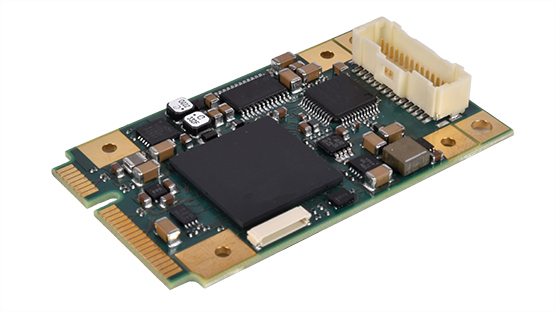
\includegraphics[width=0.7\textwidth]{img/2_steuerung/goat_io397.png}
		\caption{Speedgoat – I/O Module 397 \cite{speedgoat:IO397_50k}}
		\label{IO397_50k:img:Module}
	\end{center}
\end{figure}
\pagebreak[1]

\subsubsection{Pin Mapping – IO397-50k}


Das Terminal Board A ist für die Verarbeitung analoger Signale konzipiert, sowohl für Eingänge als auch für Ausgänge. Die Tabelle \ref{IO397_50k:tab:Board_A} zeigt das Pin-Mapping von Terminal Board A. Dieses Board verfügt über Anschlüsse für insgesamt vier analoge Eingänge (Pins A1 bis A8) und vier analoge Ausgänge (Pins A9 bis A12). Die Ausgänge sind an einen Digital-zu-Analog-Wandler (DAC) angeschlossen, während die Eingänge mit einem Analog-zu-Digital-Wandler (ADC) verbunden sind.

\pagebreak[1]
\begin{table}[!ht]
	\centering
	\caption{IO397-50k Pin Mapping – Terminal Board A: analog I/O \cite{speedgoat:IO397_50k}}
	\label{IO397_50k:tab:Board_A}
	\begin{tabular}{lll}
		\hline
		\textbf{Pin}             & \textbf{Funktionalität} & \textbf{Type} \\ \hline
		\multicolumn{1}{l|}{A1}  & Analog input 1 +        & ADC           \\
		\multicolumn{1}{l|}{A2}  & Analog input 1 -        & ADC           \\
		\multicolumn{1}{l|}{A3}  & Analog input 2 +        & ADC           \\
		\multicolumn{1}{l|}{A4}  & Analog input 2 -        & ADC           \\
		\multicolumn{1}{l|}{A5}  & Analog input 3 +        & ADC           \\
		\multicolumn{1}{l|}{A6}  & Analog input 3 -        & ADC           \\
		\multicolumn{1}{l|}{A7}  & Analog input 4 +        & ADC           \\
		\multicolumn{1}{l|}{A8}  & Analog input 4 -        & ADC           \\ \hline
		\multicolumn{1}{l|}{A9}  & Analog output 1         & DAC           \\
		\multicolumn{1}{l|}{A10} & Analog output 2         & DAC           \\
		\multicolumn{1}{l|}{A11} & Analog output 3         & DAC           \\
		\multicolumn{1}{l|}{A12} & Analog output 4         & DAC           \\ \hline
		\multicolumn{1}{l|}{A13} & GND                     & GND           \\
		\multicolumn{1}{l|}{A14} & GND                     & GND           \\
		\multicolumn{1}{l|}{A15} & 0 V                     & 0 V           \\
		\multicolumn{1}{l|}{A16} & 5 V DC                  & 5 V DC        \\
		\multicolumn{1}{l|}{A17} & GND                     & GND           \\
		\multicolumn{1}{l|}{SH}  & SH                      & Shielding     \\ \hline
	\end{tabular}
\end{table}
\pagebreak[1]


Terminal Board B hingegen bietet eine flexible Konfiguration für digitale Ein- und Ausgänge. Die Tabelle \ref{IO397_50k:tab:Board_B} zeigt das Pin Mapping von Terminal Board B. Die Pins B3 bis B16 sind für konfigurierbare I/O-Funktionalitäten ausgelegt und nutzen TTL-Signale (Transistor-Transistor-Logik), was sie besonders für schnelle digitale Schaltvorgänge geeignet macht. Dieses Board ermöglicht es, die Anschlüsse flexibel zu nutzen, je nach den Anforderungen der Applikation. Auch hier gibt es mehrere Spannungs- und Ground-Anschlüsse, sowie eine Abschirmung (Shielding) für das M12-Kabel, um elektromagnetische Störungen zu minimieren.


\pagebreak[1]
\begin{table}[!ht]
	\centering
	\caption{IO397-50k Pin Mapping – Terminal Board B: analog I/O \cite{speedgoat:IO397_50k}}
	\label{IO397_50k:tab:Board_B}
	\begin{tabular}{lll}
		\hline
		\textbf{Pin}             & \textbf{Funktionalität} & \textbf{Type} \\ \hline
		\multicolumn{1}{l|}{B1}  & 0 V                     & 0 V           \\
		\multicolumn{1}{l|}{B2}  & 5 V DC                  & 5 V DC        \\ \hline
		\multicolumn{1}{l|}{B3}  & I/O 0                   & IN/OUT        \\
		\multicolumn{1}{l|}{B4}  & I/O 1                   & IN/OUT        \\
		\multicolumn{1}{l|}{B5}  & I/O 2                   & IN/OUT        \\
		\multicolumn{1}{l|}{B6}  & I/O 3                   & IN/OUT        \\
		\multicolumn{1}{l|}{B7}  & I/O 4                   & IN/OUT        \\
		\multicolumn{1}{l|}{B8}  & I/O 5                   & IN/OUT        \\
		\multicolumn{1}{l|}{B9}  & I/O 6                   & IN/OUT        \\
		\multicolumn{1}{l|}{B10} & I/O 7                   & IN/OUT        \\
		\multicolumn{1}{l|}{B11} & I/O 8                   & IN/OUT        \\
		\multicolumn{1}{l|}{B12} & I/O 9                   & IN/OUT        \\
		\multicolumn{1}{l|}{B13} & I/O 10                  & IN/OUT        \\
		\multicolumn{1}{l|}{B14} & I/O 11                  & IN/OUT        \\
		\multicolumn{1}{l|}{B15} & I/O 12                  & IN/OUT        \\
		\multicolumn{1}{l|}{B16} & I/O 13                  & IN/OUT        \\\hline
		\multicolumn{1}{l|}{B17} & GND                     & GND           \\
		\multicolumn{1}{l|}{B18} & SH                      & Shielding     \\ \hline
	\end{tabular}
\end{table}
\pagebreak[4]


\subsubsection{IO397-50k – Konfigurieren}
\label{Simulink:IO397_50k_Konfigurieren}

Der Driver Block, wie in Abbildung \ref{IO397_50k_Konfigurieren:img:Driver_Block} gezeigt, können an dem Pull-Widerstand des I/O-Moduls verschiedne Spannungen eingestellt werden. Zur Auswahl stehen:
\begin{itemize}
	\item Pull-up 3,3 V
	\item Weak Pull-up 5,0 V
	\item Pull-down
	\item Floating
\end{itemize}
welche im Folgenden erklärt werden.

\pagebreak[1]
\begin{figure}[!ht]
	\begin{center}
		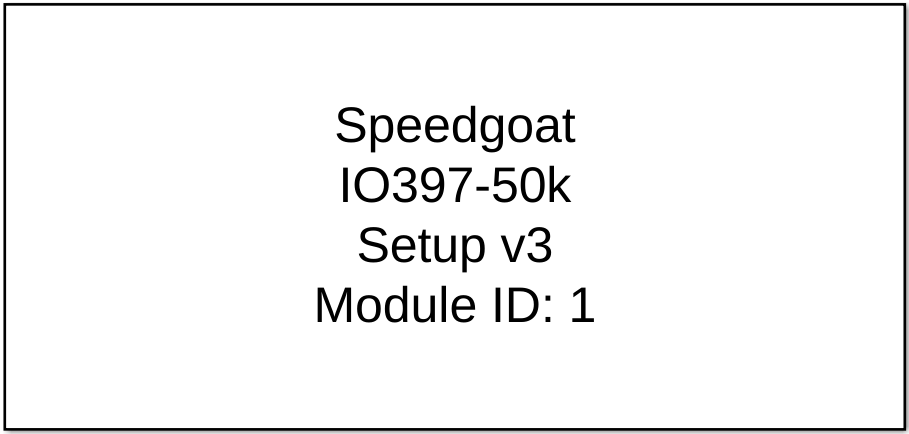
\includegraphics[width=.5\textwidth]{img/4_simulink/IO397_50k.png}
		\caption{Simulink – Driver Block – IO397-50k}
		\label{IO397_50k_Konfigurieren:img:Driver_Block}
	\end{center}
\end{figure}
\pagebreak[1]

Pull-Widerstände werden verwendet, um klare digitale Schaltzustände zu gewährleisten. Es gibt drei verschiedene Zustände: High entspricht logisch 1, Low entspricht logisch 0 und Floating ist hochohmig. Die Zustände zu den Einstellungen sind in der Tabelle \ref{IO397_50k_Konfigurieren:tab:Reaktionszeit} aufgeführt.
In Abbildung \ref{IO397_50k_Konfigurieren:img:TTL_IO_Interface} ist im rot markierten Bereich der Pull-Widerstand mit 4,7 k$\Omega$ an einen 47-$\Omega$-Widerstand am I/O-Anschluss angeschlossen. Der Pull-Widerstand kann, wie bereits erwähnt, konfiguriert werden. Dabei wird intern am Pull-Widerstand entweder eine Spannung von 3,3 V, 5 V, GND oder kein Kontakt, also Floating (hochohmig), geschaltet.

\pagebreak[1]
\begin{figure}[!ht]
	\begin{center}
		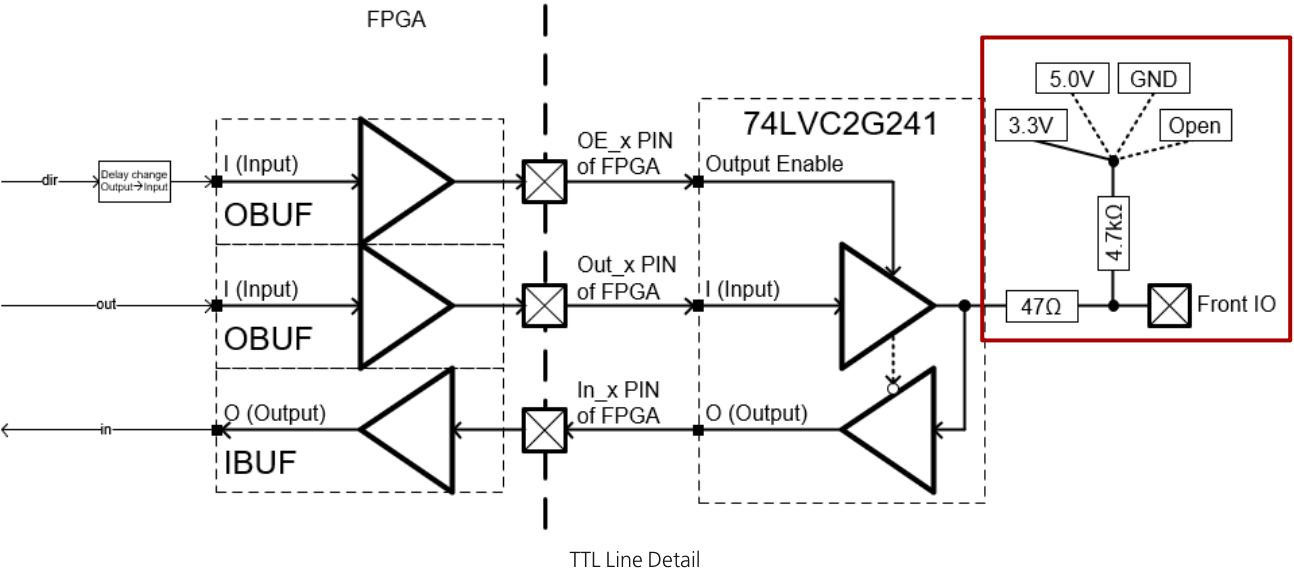
\includegraphics[width=1.1\textwidth]{img/4_simulink/TTL_IO_Interface.png}
		\caption{Simulink – TTL I/O Interface – IO397-50k \cite[12]{speedgoat:IO397_50k}}
		\label{IO397_50k_Konfigurieren:img:TTL_IO_Interface}
	\end{center}
\end{figure}
\pagebreak[4]



Bei der Einstellung auf 3,3 V oder 5 V fungiert der Widerstand als Pull-up-Widerstand. Bei der Pull-down-Konfiguration liegt am Widerstand Ground (GND) an.



In Tabelle \ref{IO397_50k_Konfigurieren:tab:Reaktionszeit} können die Reaktionszeiten der digitalen Ausgänge verglichen werden. Bei der Einstellung Weak Pull-up 5,0 V bedeutet \frqq weak\flqq, dass der Ausgang eine langsamere Anstiegszeit hat. In Abbildung \ref{IO397_50k_Konfigurieren:img:Pull_Widerstande} sind die Reaktionszeiten dargestellt.


\pagebreak[1]
\begin{table}[!ht]
	\centering
	\caption{Simulink – Pull-Widerstand – Reaktionszeit}
	\label{IO397_50k_Konfigurieren:tab:Reaktionszeit}
	\begin{tabular}{lccc}
		\hline
		\multicolumn{1}{c}{\multirow{2}{*}{\textbf{Einstellung}}} & \multicolumn{1}{c}{\multirow{2}{*}{\textbf{Logischer zustand}}} & \multicolumn{2}{c}{\textbf{Reaktionszeit der Ausgänge}}           \\ \cline{3-4}
		\multicolumn{1}{c}{}                                      & \multicolumn{1}{c}{}                                            & Anstieg                                                 & Abfall  \\ \hline
		\multicolumn{1}{l|}{Pull-up 3,3V}                         & I/O = 1                                                         & Schnell                                                 & Schnell \\
		\multicolumn{1}{l|}{weak pull-up 5,0V}                    & I/O = 1                                                         & Langsam                                                 & Schnell \\
		\multicolumn{1}{l|}{Pull-down}                            & I/O = 0                                                         & Schnell                                                 & Langsam \\
		\multicolumn{1}{l|}{Floating}                             & I/O = 0 -1                                                      & -                                                       & -       \\ \hline
	\end{tabular}
\end{table}
\pagebreak[1]



\pagebreak[1]
\begin{figure}
	\begin{minipage}{0.8\textwidth}
		\centering
		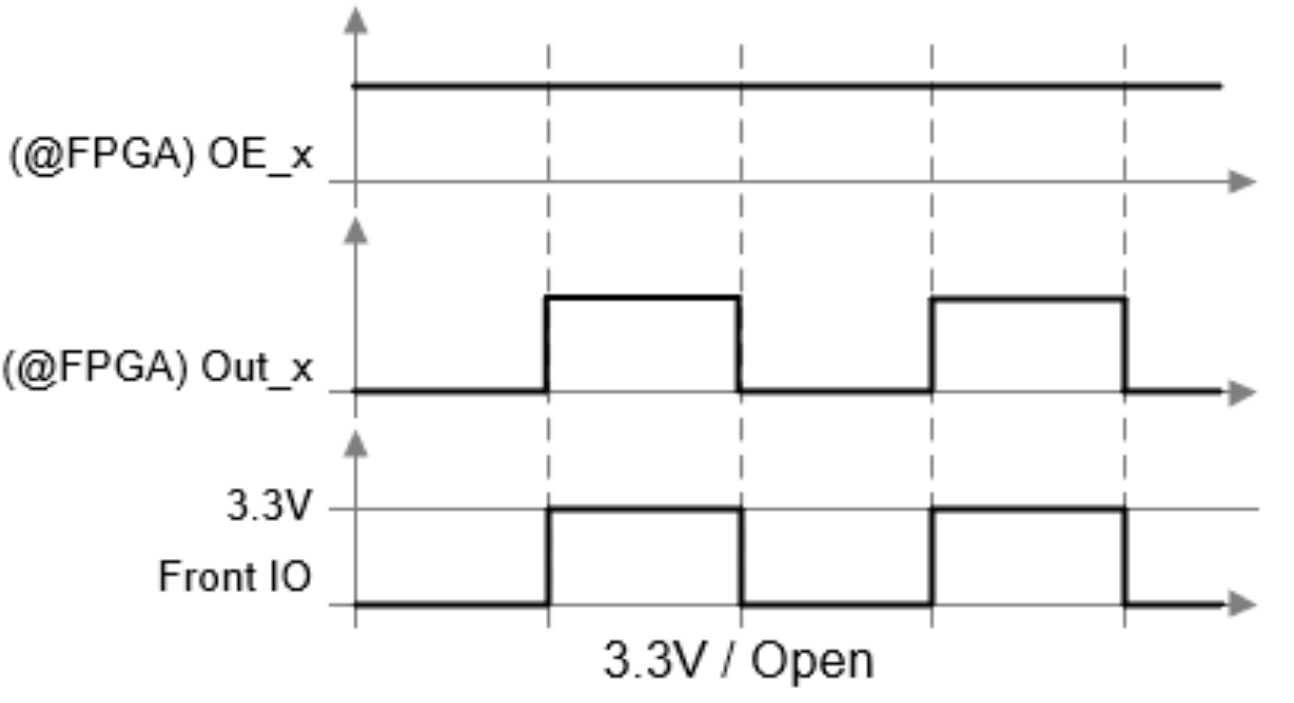
\includegraphics[width=1\textwidth]{img/4_simulink/O_Interface_3V3.png}
		\caption*{Pull-up-Widerstand 3,3 V}
	\end{minipage}
	\begin{minipage}{0.8\textwidth}
		\centering
		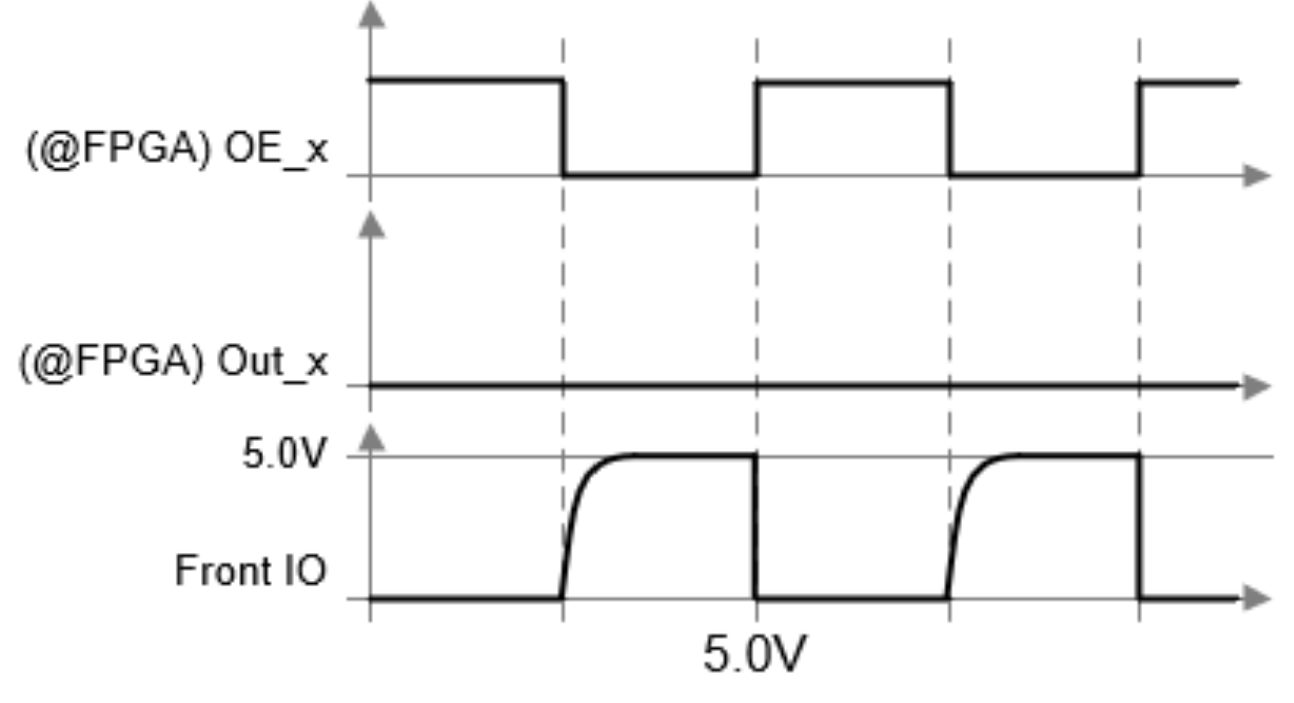
\includegraphics[width=1\textwidth]{img/4_simulink/O_Interface_5V.png}
		\caption*{Weak Pull-up-Widerstand 5 V}
	\end{minipage}
	\begin{minipage}{0.8\textwidth}
		\centering
		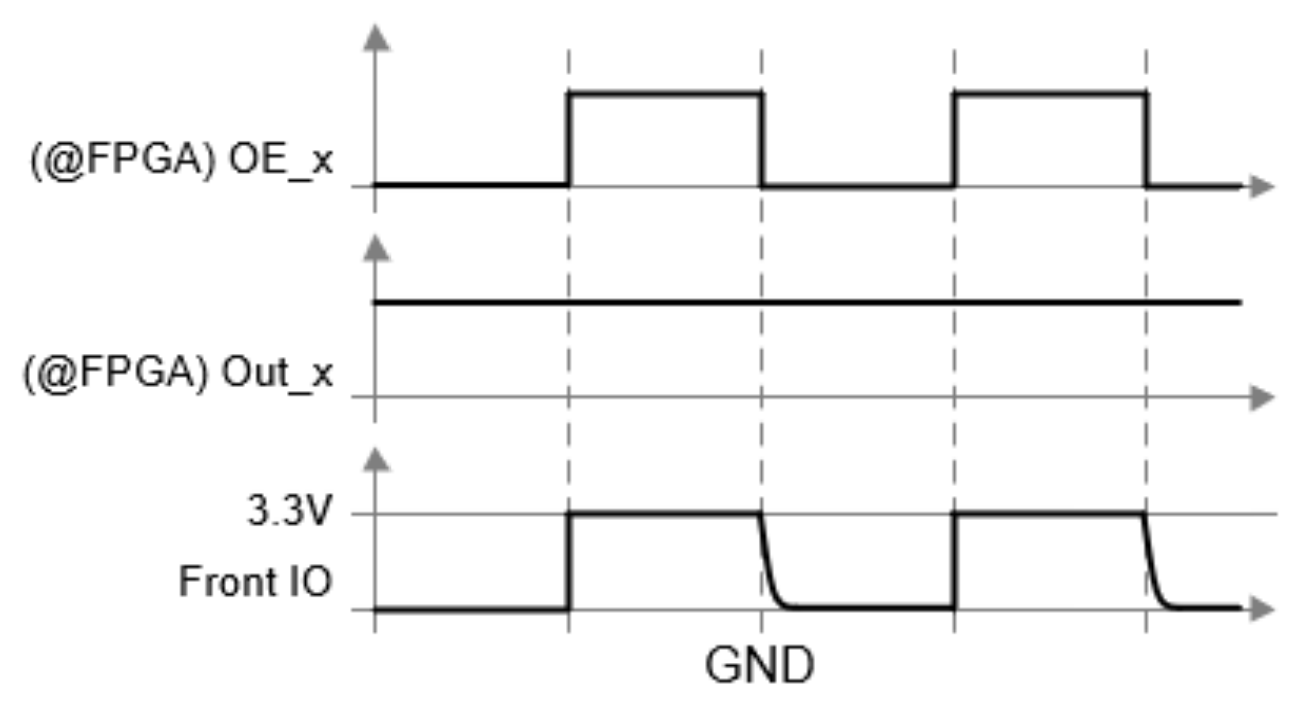
\includegraphics[width=1\textwidth]{img/4_simulink/O_Interface_0V.png}
		\caption*{Pull-down-Widerstand GND}
	\end{minipage}
	\caption{Simulink – Pull-Widerstände – IO397-50k \cite[12]{speedgoat:IO397_50k}}
	\label{IO397_50k_Konfigurieren:img:Pull_Widerstande}
\end{figure}
\pagebreak[4]

\newpage
\subsection{I/O-Modul – IO691}
\label{section:IO691}

Das IO691 I/O-Modul bietet eine intelligente CAN-Schnittstelle mit zwei Kanälen, die sowohl flexible Datenrate CAN (CAN FD) als auch High-Speed CAN (CAN HS) unterstützen. Es ist kompatibel mit CAN 2.0A/B-Netzwerken und unterstützt SAE J1939 sowie ASAM XCP für Bypassing. Alle Signale sind über 9-polige D-Sub-Front-CAN-Anschlüsse zugänglich \cite{speedgoat:IO691}.

\pagebreak[1]
\begin{figure}[!ht]
	\begin{center}
		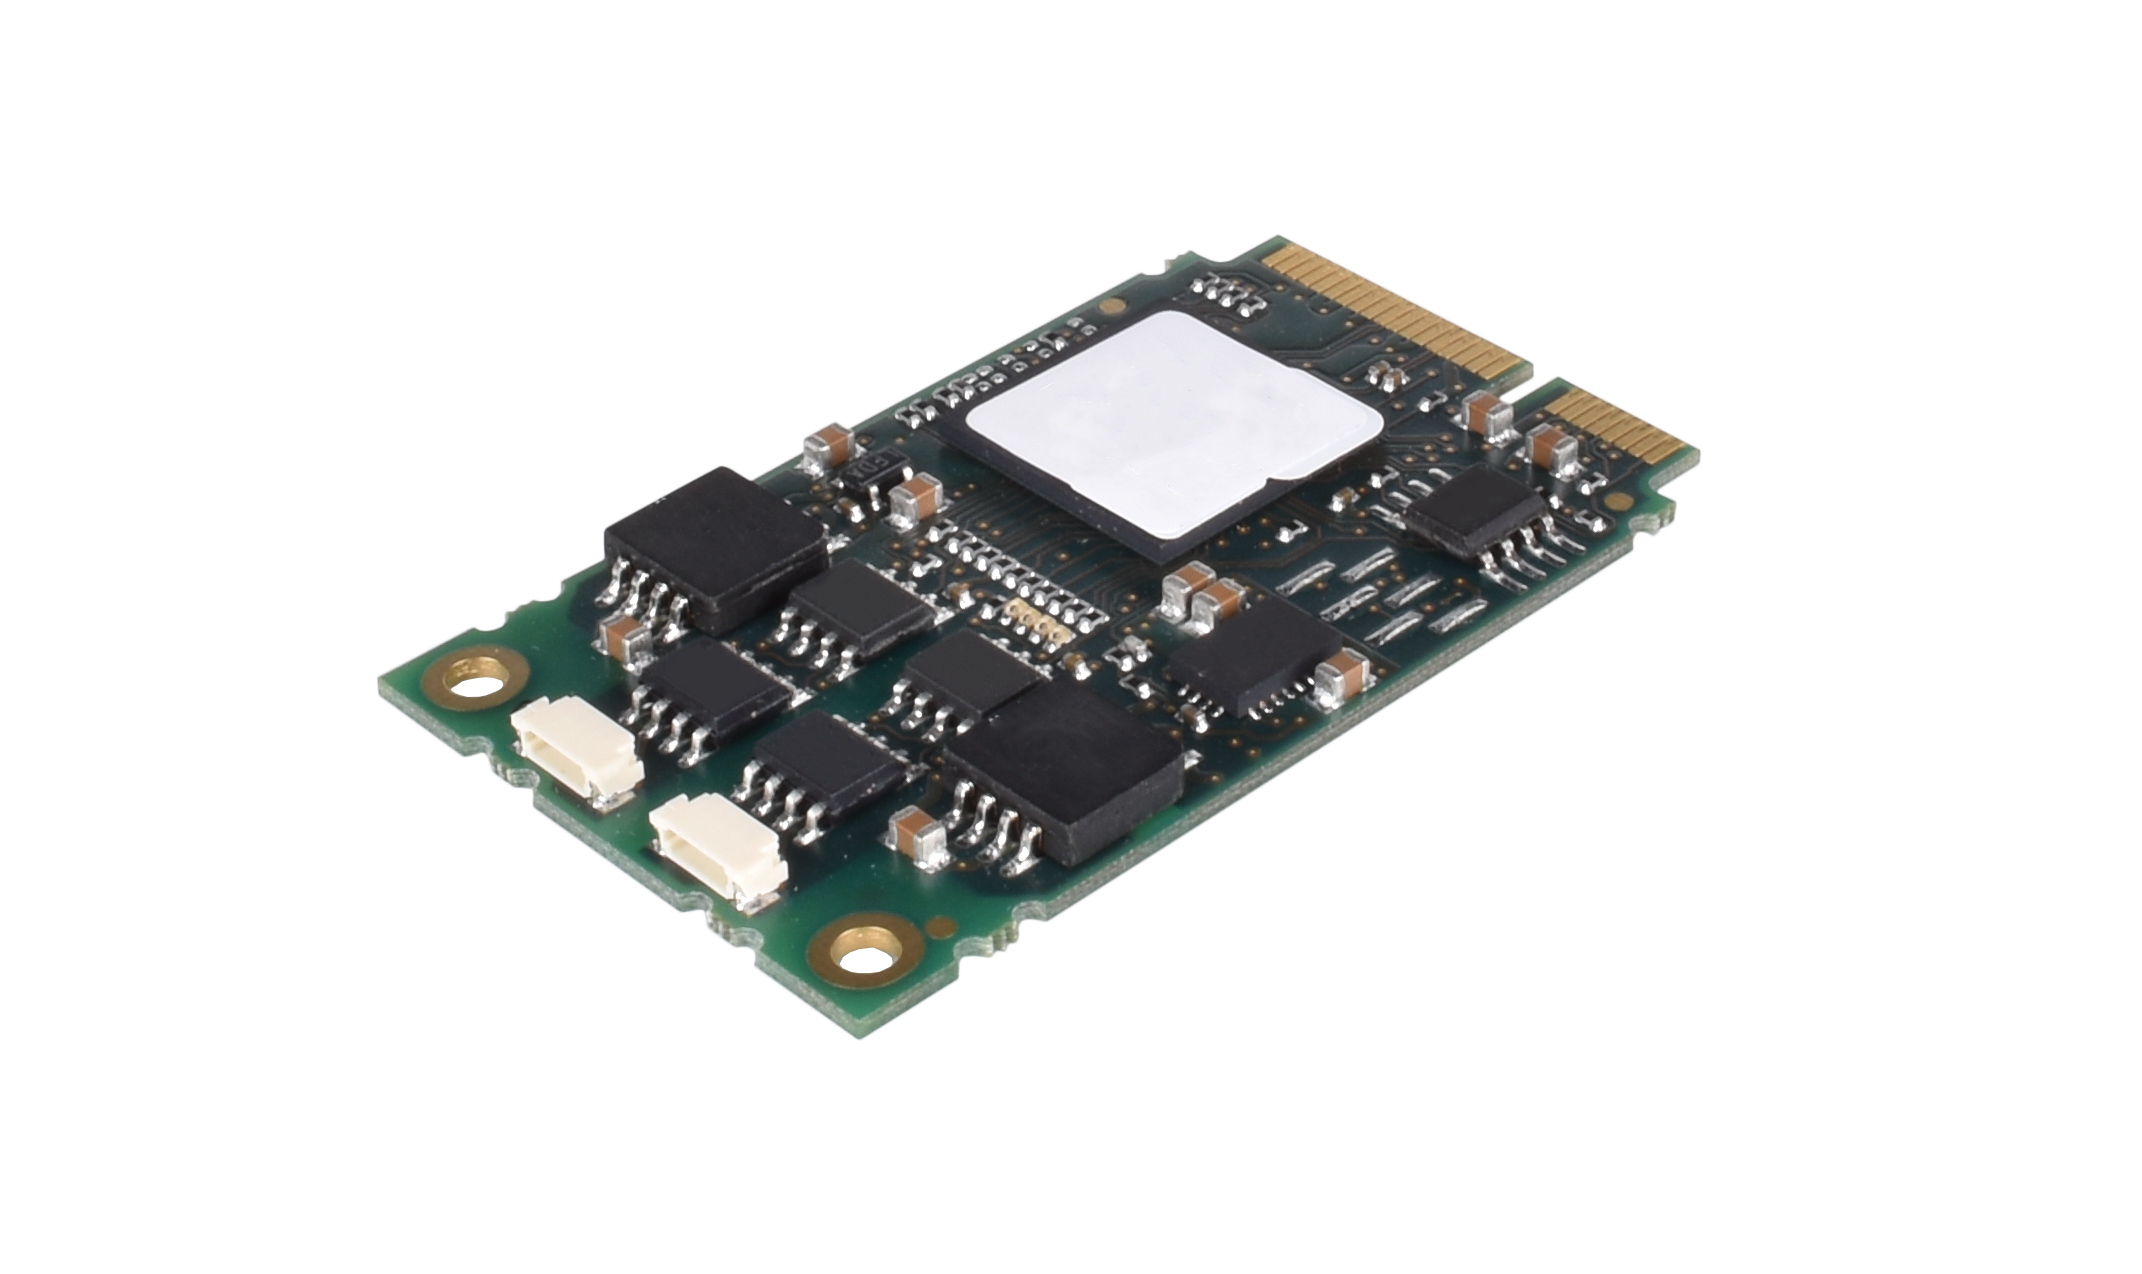
\includegraphics[width=0.7\textwidth]{img/2_steuerung/goat_io691.png}
		\caption{Speedgoat – I/O Module 691 \cite{speedgoat:IO691}}
		\label{img_2_2:goat:IO691}
	\end{center}
\end{figure}
\pagebreak[4]




\subsubsection{Pin Mapping –  IO691}

\pagebreak[1]
\begin{table}[!ht]
	\centering
	\caption{IO691 Pin Mapping}
	\label{speedgoat:IO691}
	\begin{tabular}{ll}
		\hline
		\textbf{Pin}           & \textbf{DB9 Connector A/B, Signal} \\ \hline
		\multicolumn{1}{l|}{1} & -                                  \\
		\multicolumn{1}{l|}{2} & CAN-low                            \\
		\multicolumn{1}{l|}{3} & GND                                \\
		\multicolumn{1}{l|}{4} & -                                  \\
		\multicolumn{1}{l|}{5} & -                                  \\
		\multicolumn{1}{l|}{6} & GND                                \\
		\multicolumn{1}{l|}{7} & CAN-high                           \\
		\multicolumn{1}{l|}{8} & -                                  \\
		\multicolumn{1}{l|}{9} & -                                  \\ \hline
	\end{tabular}
\end{table}
\pagebreak[4]


\subsubsection{IO691 Module Konfigurieren}
\label{Simulink:IO691_Konfigurieren}


\newpage
\section{Simulink}
\label{section:Simulink}

\myboxy{
	\begin{itemize}
		\item
	\end{itemize}
}{To-do}{\textwidth}



\newpage
\section{QElectroTech}
\label{section:QElectroTech}

\myboxy{
	\begin{itemize}
		\item
	\end{itemize}
}{To-do}{\textwidth}




\chapter{Bonusmaterial}
\label{sec:Anhang}

\chapter{Implementierung}

\section{Bauteile}

Für das Projekt wurden die echtzeitfähige Steuerung, die Batterie, der Motor und die zugehörige Steuerung vorgegeben. Alle weiteren Bauteile mussten bestellt werden.

\section{Schaltplan}




\myboxy{
	\begin{itemize}
		\item Funktion (=Anlage) und Ortskennzeichen (+Ort) definieren. Funktionales Engineering.
		\item Bauteilkennzeichnung (BMK) festlegen.
		\item Aderfarben und Querschnitt definieren.
		\item Ausgewählte Bauteile in die Schaltung integrieren.
		\item Nicht vorhandene Bauteile selbst erstellen.
		      \begin{itemize}
			      \item Bauteile sortiert hinzufügen: Spannungsversorgung, Steuerung (Eingang, dann Ausgang), Lastkreis und Sonderfunktionen.
		      \end{itemize}
	\end{itemize}}{To-do}{\textwidth}





Zu Beginn der Erstellung des Schaltplans sollten die Funktions- und Ortskennzeichen, sowie die Beschriftung der Bauteile und Leitungen festgelegt werden. Die Verdrahtung erfordert die Zuordnung von Aderfarben, die den jeweiligen Potenzialen entsprechen.

\subsection{Betriebsmittelbezeichnung}

Ein Betriebsmittel besteht aus verschiedenen Kennzeichen: dem Funktionskennzeichen (=), dem Ortskennzeichen (+) und dem Betriebsmittelkennzeichen (-). Früher wurde das Funktionskennzeichen als „Anlage“ bezeichnet. In der neuen DIN EN IEC 81346-2 \cite{DIN_EN_IEC_81346-2} wurde diese Bezeichnung jedoch auf „Funktion“ geändert.

Das Funktionskennzeichen beschreibt eine bestimmte Funktion im Schaltplan, wie beispielsweise die Spannungsversorgung oder die Steuerung (siehe Tabelle \ref{bmk:funktionskennzeichen}).

\begin{table}[!ht]
	\centering
	\caption{Schaltplan – Funktionskennzeichen (=)}
	\label{bmk:funktionskennzeichen}
	\begin{tabular}{ll}
		\hline
		\textbf{Abkürzung}      & \textbf{Bezeichnung} \\ \hline
		\multicolumn{1}{l|}{SV} & Spannungsversorung   \\
		\multicolumn{1}{l|}{ES} & Eingänge Steuerung   \\
		\multicolumn{1}{l|}{AS} & Ausgänge Steuerung   \\
		\multicolumn{1}{l|}{KO} & Kommunikation        \\
		\multicolumn{1}{l|}{AT} & Antrieb              \\
		\multicolumn{1}{l|}{NA} & Not-Aus              \\ \hline
	\end{tabular}
\end{table}

Das Ortskennzeichen gibt an, an welchem Ort ein Bauteil installiert ist. Beispielsweise gibt es im Pod eine Steuereinheit und eine Batterieeinheit. Im Schaltplan wird dadurch deutlich, welche Verbindungen zwischen verschiedenen Orten bestehen. Das Ortskennzeichen erleichtert zudem die Wartung und Installation des Systems.

\begin{table}[!ht]
	\centering
	\caption{Schaltplan – Ortskennzeichen (+)}
	\label{bmk:ortskennzeichen}
	\begin{tabular}{ll}
		\hline
		\textbf{Abkürzung}       & \textbf{Bezeichnung} \\ \hline
		\multicolumn{1}{l|}{POD} & Fahrzeug             \\
		\multicolumn{1}{l|}{BE}  & Batterieeinheit      \\
		\multicolumn{1}{l|}{SE}  & Steuereinheit        \\
		\multicolumn{1}{l|}{AE}  & Antriebseinheit      \\ \hline
	\end{tabular}
\end{table}


\begin{figure}[!ht]
	\begin{center}
		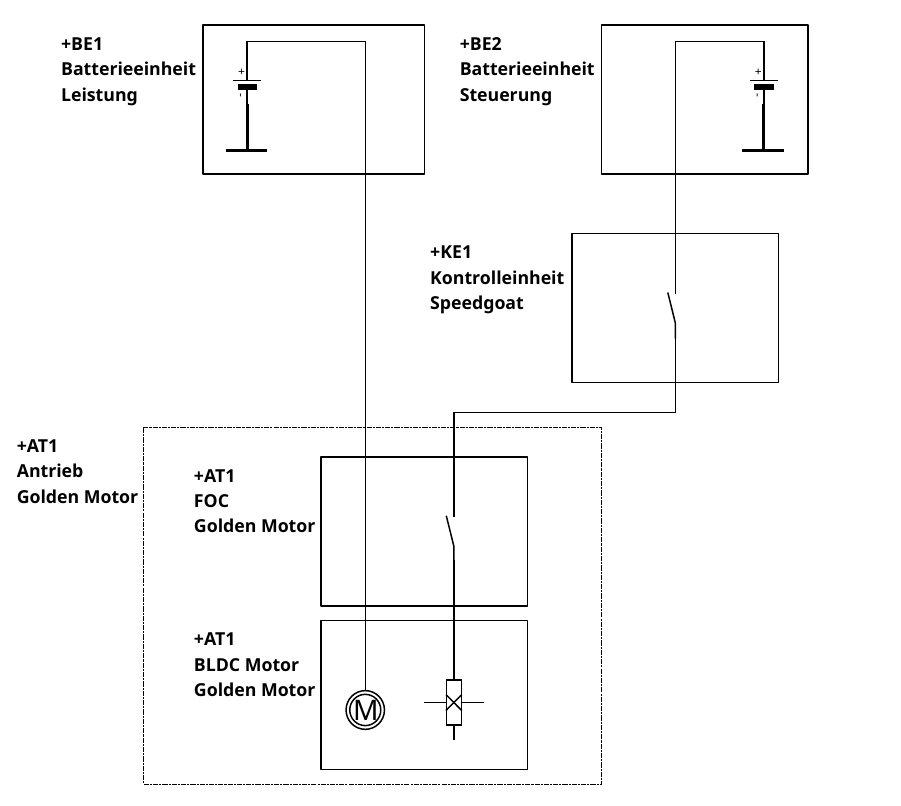
\includegraphics[width=1\textwidth]{img/3_schaltplan/sp_aufbauplan_1.png}
		\caption{Schaltplan – Aufbauplan}
		\label{img_3_2:aufbauplan:1}
	\end{center}
\end{figure}


Das Betriebsmittelkennzeichen bezeichnet das spezifische Bauteil. Die genaue Zuordnung der Bezeichnungen ist in der DIN EN IEC 81346-2 geregelt. Die für das Projekt relevanten Betriebsmittelkennzeichen sind in Tabelle \ref{bmk:betriebsmittelkennzeichen} aufgeführt.

Bei einer vollständigen Betriebsmittelbezeichnung sieht das Kennzeichen des Betriebsmittels wie folgt aus: =SA+KE-KE101, Bei der .

\begin{table}[!ht]
	\centering
	\caption{Schaltplan – Betriebsmittelkennzeichen (-) \cite{DIN_EN_IEC_81346-2}}
	\label{bmk:betriebsmittelkennzeichen}
	\begin{tabular}{|l|lll|}
		\hline
		\textbf{Abkürzung}       & \textbf{Klassenname}                            & \multicolumn{1}{l|}{\textbf{Allgemeine Bedeutung}} \\ \hline
		\multicolumn{1}{|l|}{FC} & \makecell[l]{Überstromschutzobjekt}             & \multicolumn{1}{l|}{Sicherung}                     \\ \hline
		\multicolumn{1}{|l|}{GB} & \makecell[l]{Erzeugungsobjekt für elektrische                                                        \\Energie durch chemische Energie} & \multicolumn{1}{l|}{Batterie} \\ \hline
		\multicolumn{1}{|l|}{KE} & \makecell[l]{Elektrische Signale                                                                     \\verarbeitendes Objekt}   & \multicolumn{1}{l|}{Steuerung} \\ \hline
		\multicolumn{1}{|l|}{MA} & \makecell[l]{Elektromagnetisches                                                                     \\Rotationsantriebsobjekt} & \multicolumn{1}{l|}{Motor} \\ \hline
		\multicolumn{1}{|l|}{QA} & \makecell[l]{Stromsteuerungsobjekt}             & \multicolumn{1}{l|}{Relais}                        \\ \hline
		\multicolumn{1}{|l|}{RL} & \makecell[l]{Bewegungsbegrenzungsobjekt}        & \multicolumn{1}{l|}{Bremse}                        \\ \hline
		\multicolumn{1}{|l|}{SF} & \makecell[l]{Gesichtsinteraktionsobjekt}        & \multicolumn{1}{l|}{Schalter}                      \\ \hline
		\multicolumn{1}{|l|}{TB} & \makecell[l]{Stromkonvertierungsobjekt}         & \multicolumn{1}{l|}{Transformator}                 \\ \hline
		\multicolumn{1}{|l|}{WD} & \makecell[l]{Niederspannungsenergie Leitobjekt} & \multicolumn{1}{l|}{Leitung/Kabel}                 \\ \hline
		\multicolumn{1}{|l|}{XD} & \makecell[l]{Niederspannungs-Verbindungsobjekt} & \multicolumn{1}{l|}{Klemme, Stecker oder Buchse}   \\ \hline
	\end{tabular}
\end{table}




\newpage

\subsection{Bauteilerstellung}

In der Software QElectroTech, kann dies in der Bauteilsammlung getan werden.


\section{Distanzmessung}

\myboxy{
	\begin{itemize}
		\item + Anschlüsse herauszufinden vier anschlüsse gefunden.
		\item + Was für Aufgaben haben die Anschlüsse?
		      \subitem Was für ein Kommunikationsprotokol hat der Sensor?
		      \subitem Asynchron und seriell mit Baudrate 115200. (Ozilloskop)
		\item mit einem ESP32 die Sensordaten lesen.
		\item Nachrichtdekodierung (Controller MCU)
		      \subitem Ox24 Start (Nachricht start)
		      \subitem 0x26 Stopp (Nachricht ende)
		      \subitem 24 30 30 30 33 32 36 30 30 32 39 26 (Stopp signal)
		      \subitem 24 30 30 30 33 32 36 30 31 33 30 26 (Laser an)
		      \subitem 24 30 30 30 32 32 31 32 33 26 (Messen)
	\end{itemize}}{To-do}{\textwidth}


Der Sensor von Pepperl+Fuchs wurde ursprünglich für die Distanzmessung angeschafft. Da dieser Sensor jedoch sehr teuer ist und wir nicht das Risiko eines möglichen Schadens im Vakuum eingehen wollten, wurde nach einer kostengünstigen Alternative gesucht.\\
Die Idee bestand darin, ein Entfernungsmessgerät von PARKSIDE zu verwenden und den Sensor aus dem Gerät zu entfernen. Die Messwerte werden anschließend mit einer MCU decodiert.

\subsection{Verbindung}
Der Sensor ist über ein Flachbandkabel mit der Hauptplatine verbunden, wie in Abbildung \ref{img_2_2:sen_dis_parkside:1} zu sehen ist. Auf der Hauptplatine befinden sich vier ungenutzte Lötstellen. Mithilfe eines Oszilloskops haben wir diese Lötstellen analysiert und festgestellt, dass Leitung eins eine Spannung von 3,3 V führt und Leitung vier als GND dient. Die Leitungen zwei und drei übertragen digitale Signale und fungieren als Datenleitungen.\\
Wenn zwei Leitungen für die Datenübertragung vorhanden sind, kann die Kommunikation bei einer zweiadrigen Verbindung entweder synchron oder asynchron erfolgen. Ist die Kommunikation synchron, dient eine der Leitungen als Taktleitung (Clock). Andernfalls, bei einer asynchronen Kommunikation, ist eine Leitung der Sender (TX) und die andere der Empfänger (RX). Dies ermöglicht eine Vollduplex-Übertragung.
Der Sensor komuniziert mit einem Bussystem.




\begin{figure}[ht]
	\begin{center}
		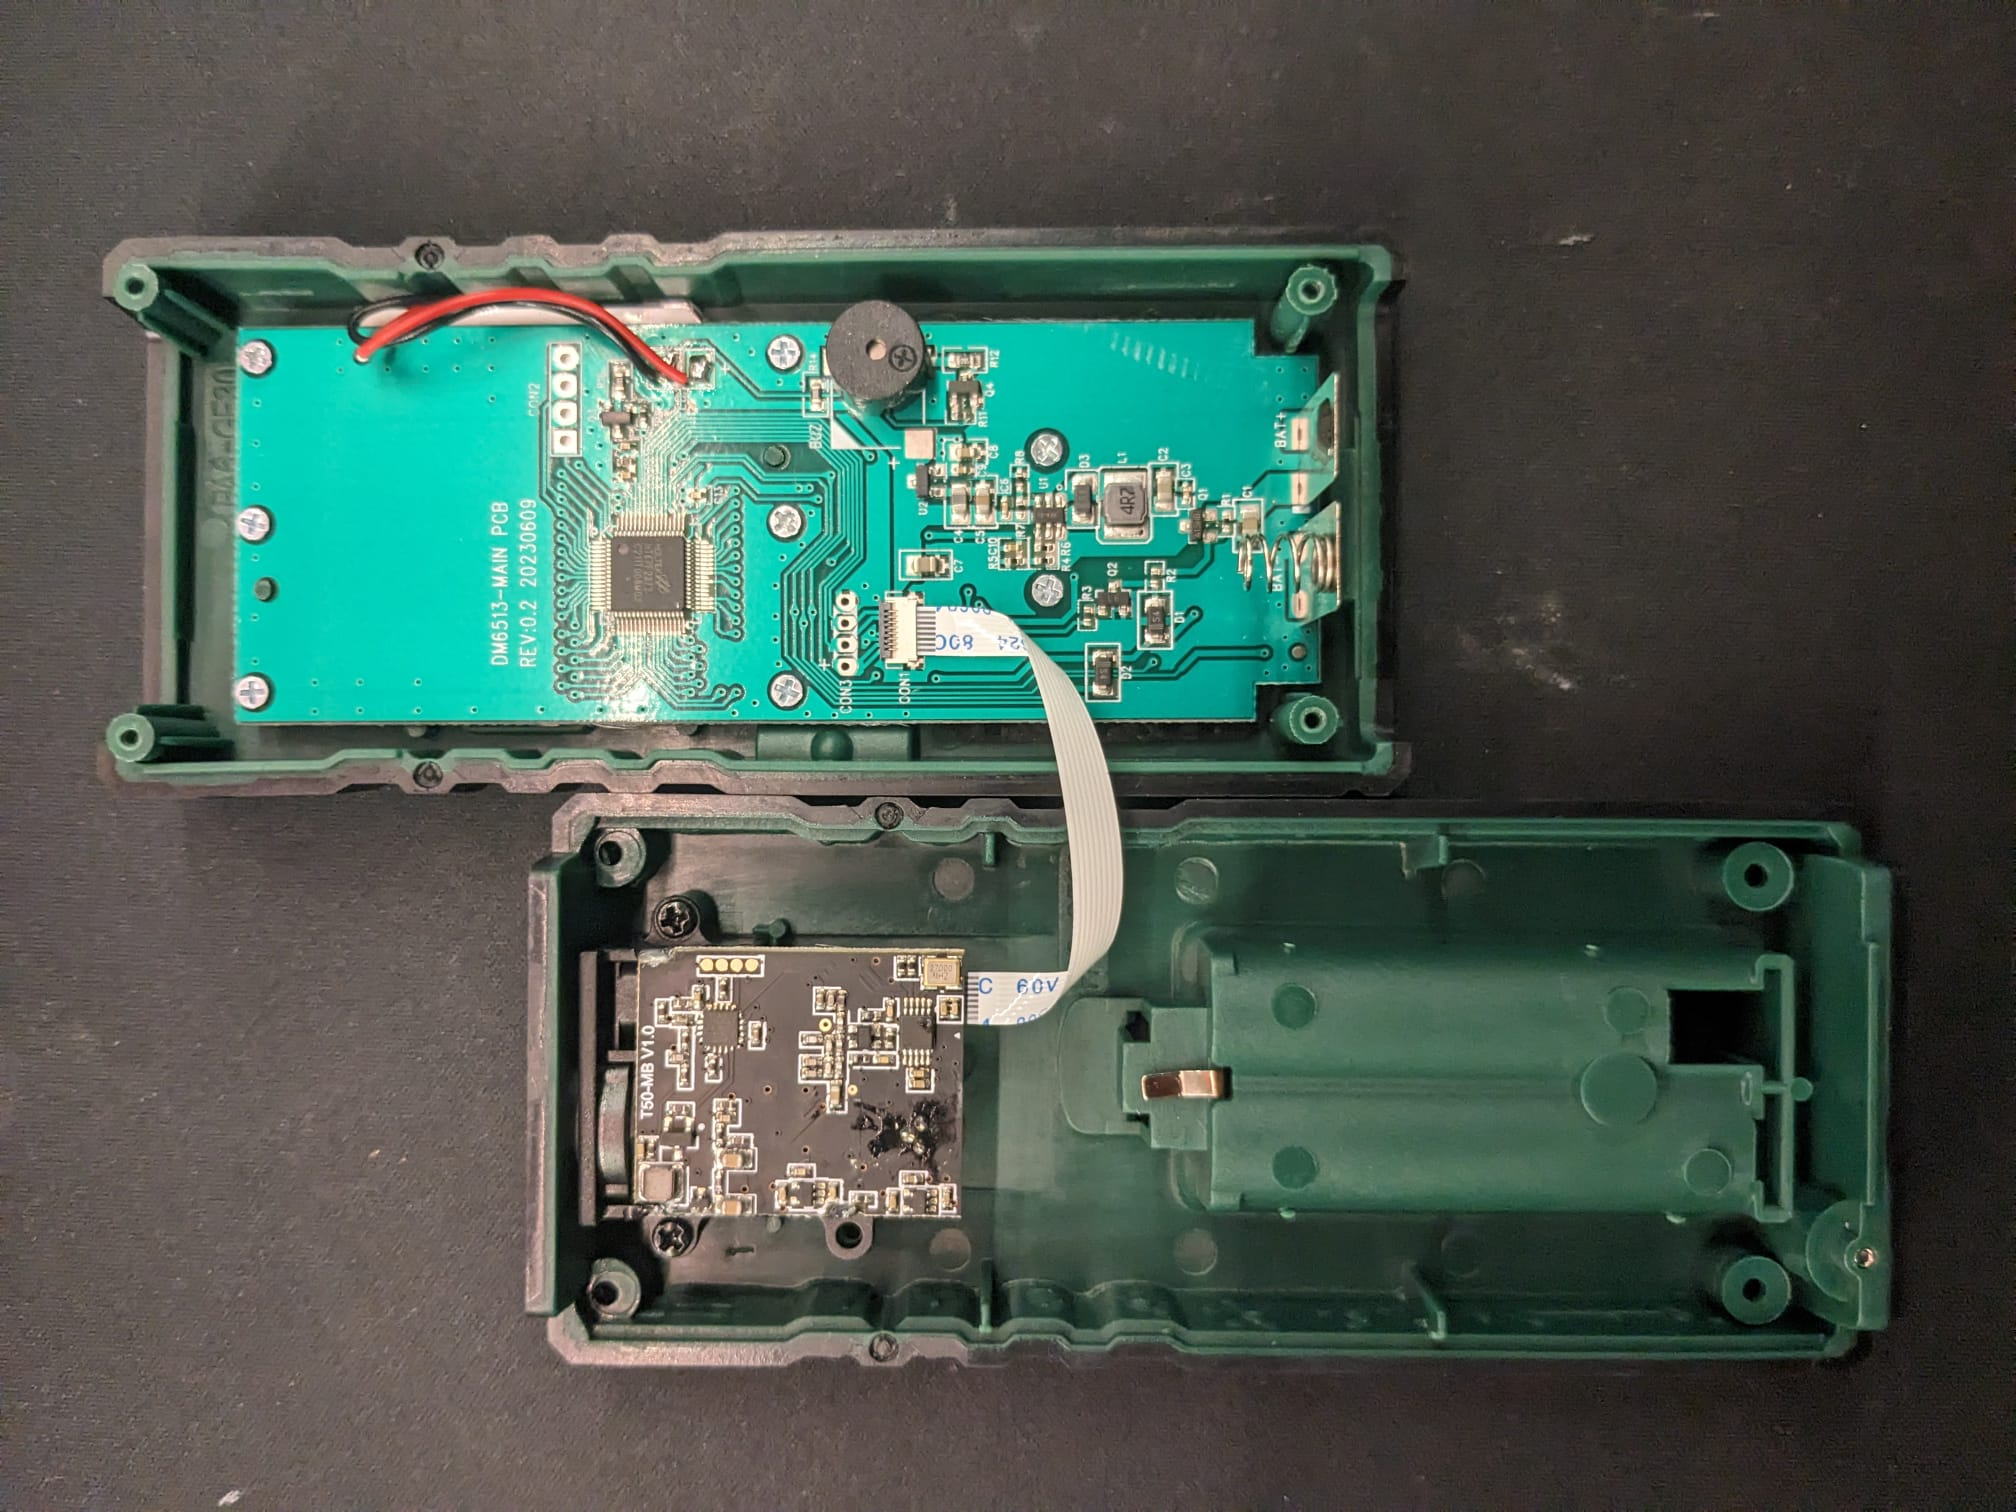
\includegraphics[width=1\textwidth]{img/2_sen/dis_parkside_1_outside.png}
		\caption{PARKSIDE – Distanzsensor – Innenaufbau}
		\label{img_2_2:sen_dis_parkside:1}
	\end{center}
\end{figure}


\begin{table}[ht]
	\centering
	\caption{PARKSIDE – Pin Mapping – Distanzsensor}
	\label{parkside:pinmapping}
	\begin{tabular}{l|ll}
		\hline
		\textbf{Pin} & \textbf{Farbe} & \textbf{Funktion} \\ \hline
		1            & Rot            & 3V3               \\
		2            & Weiß           & RX (receiver)     \\
		3            & Gelb           & TX (transmitter)  \\
		4            & Schwarz        & GND               \\ \hline
	\end{tabular}
\end{table}





\section{Steuerung}

\myboxy{
	\begin{itemize}
		\item
	\end{itemize}
}{To-do}{\textwidth}

\chapter{Bonusmaterial}
\label{sec:Anhang}

\chapter{Konklusion}
\myboxy{
	\begin{itemize}
		\item Endschnittstellen für die weiterführung des Projekts.
		\item weiterführung mit Testsenarien. 
	\end{itemize}
}{To-do}{\textwidth}
\chapter{Bonusmaterial}
\label{sec:Anhang}

\include{source/Literaturverzeichnis}
\printbibliography
\appendix
\chapter{Bonusmaterial}
\label{sec:Anhang}

\chapter{Anhang}
\section{Schaltplan}
\label{Anhang:Schaltplan}

\myboxy{
	\begin{itemize}
		\item BMK beschriftung anpassen
		\item Bauteile einpflegen
	\end{itemize}
}{To-do}{\textwidth}
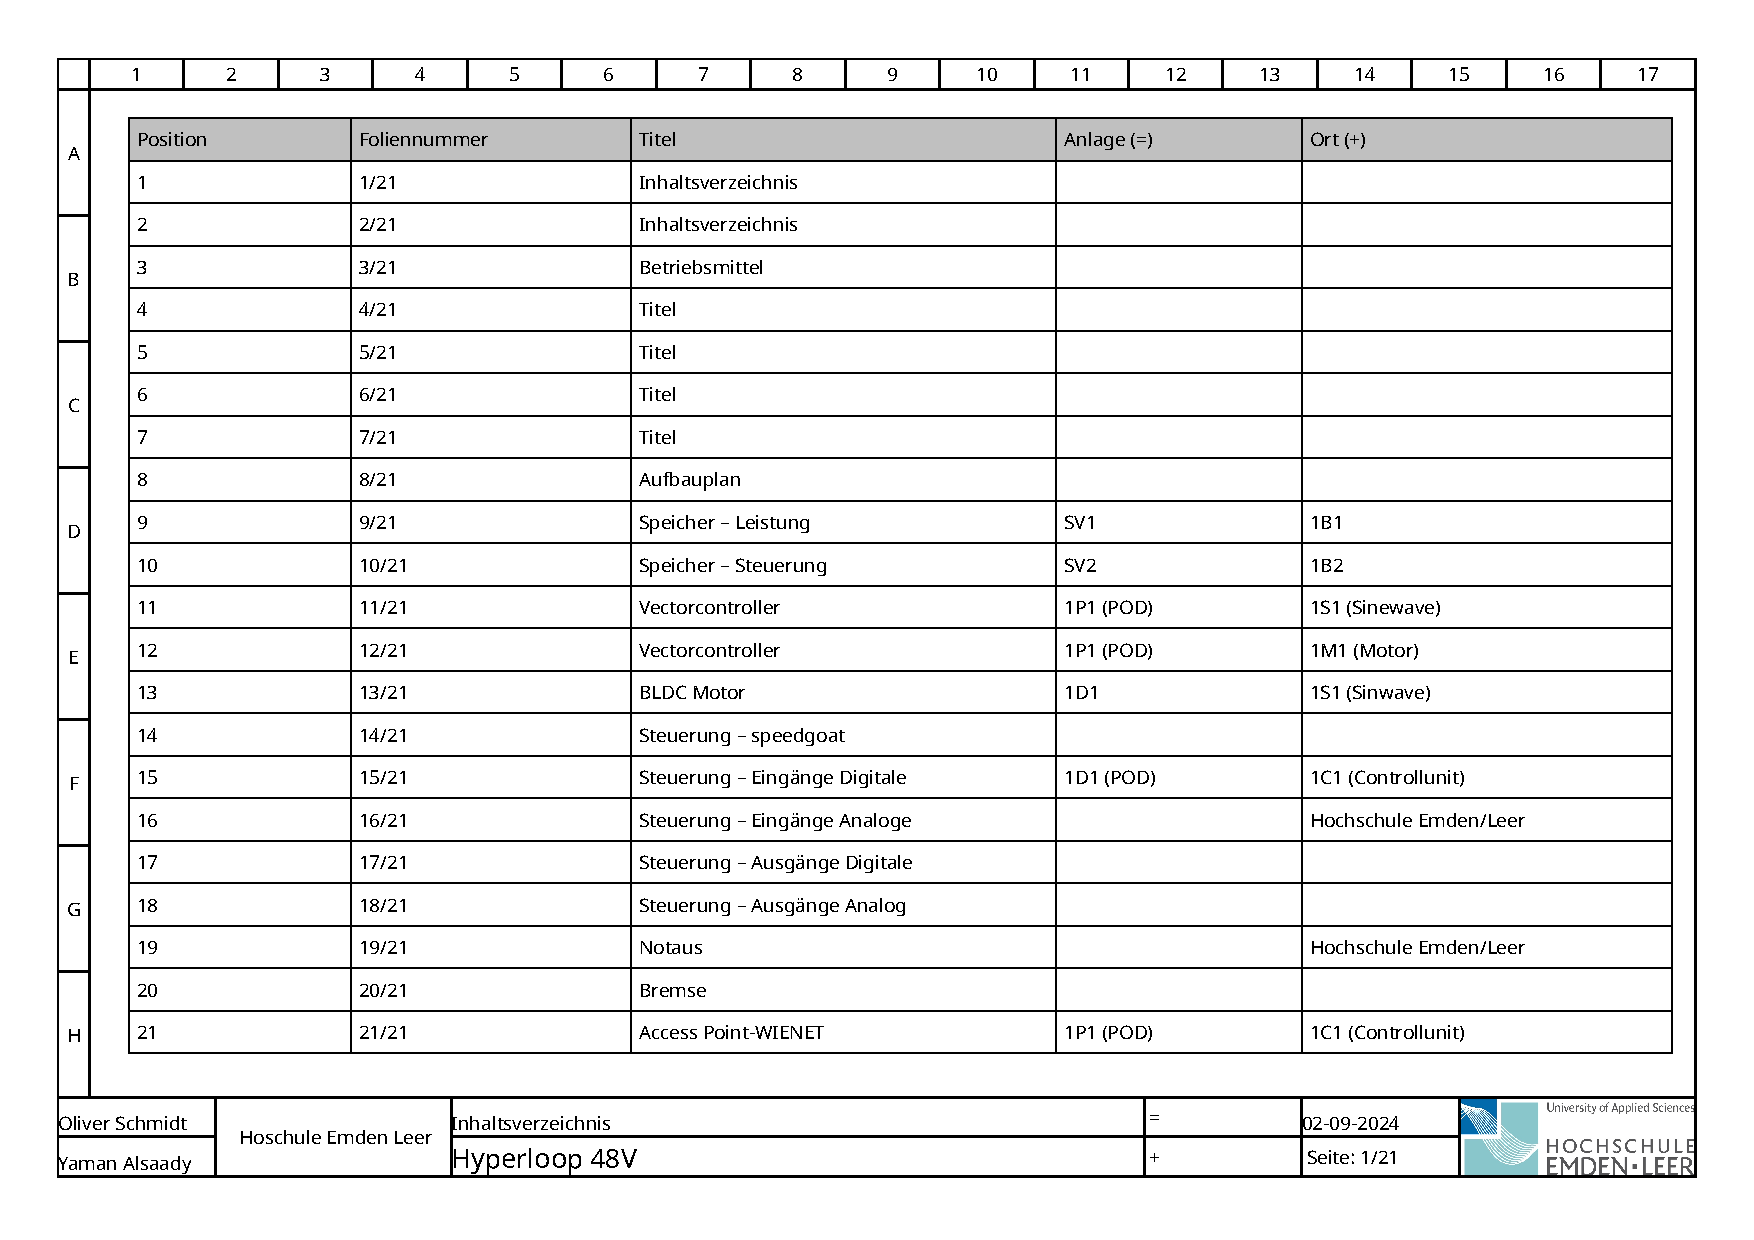
\includepdf[pages=-,landscape] {Anhang/Schaltplan.pdf}


\end{document}
